\documentclass[12pt,a4paper]{article}
\usepackage[latin1]{inputenc}
\usepackage{amsmath}
\usepackage{amsfonts}
\usepackage{amssymb}
\usepackage[pdftex]{graphicx}
\begin{document}

\begin{center}
\thispagestyle{empty}
\Large Dimensionality Reduction via Optimization\\ 
\normalsize
\vspace{80mm}
In partial fulfillment of G63.2012-002\\
New York University \\
Ross Goroshin 
\end{center}

\newpage 
\begin{center}
{\bf ABSTRACT} 
\end{center}
Most high dimensional data, such as imagery or video, can be described using many fewer parameters than the default dimensionality of the data. For instance a video of a moving object can be described by knowing the shape of the object and its configuration with respect to the camera (as opposed to the number of pixels in the image). These observations have lead to the emerging field of dimensionality reduction or manifold learning. This work deals with dimensionality reduction, particularly with a technique known as sparse coding. Sparse coding seeks to find a basis which sparsely reconstructs the data. 
\newpage
\section{Introduction} 
\begin{center} 
\textit{Entia non sunt multiplicanda praeter necessitatem.} \\
\begin{flushright} 
-Occam's razor 
\end{flushright}
\end{center}
Ever since the relatively recent explosion in computational power and storage, researchers have been attempting to replicate the life-like ability to extract key pieces of information from vast amounts of data. Most notably these tasks usually fall into to what have come to be known as the fields of pattern recognition and machine learning. One of the leading applications of these fields are in computer vision, defined as the science and technology of machines that see \cite{Encyclopedia Britannica}. Where the term "see" refers to the extraction of relevant information from imagery and video. By default, data in computer vision (as well as many other fields) is assigned a very high dimension. That is to say, each measurement is initially treated as independent from all the others because an explicit relationship is usually too difficult to obtain. For example, consider a 42 second video at a resolution of 1000 by 1000 pixels. Played at a standard rate of 24 frames per second the video contains roughly 1000 frames. Therefore the video can be represented as one thousand $10^6$ dimensional vectors, or even as a single $10^9$ dimensional vector, depending on the application. Extracting meaningful information from such high dimensional data is a challenging task for many reasons. For example, in order to answer the abstract question of "how many people are in the video?" one must find a complex relationship among the various pixels which embodies the spaciotemporal pattern that constitutes a person. One interpretation of the field of pattern recognition is to find some dependency among variables which are initially modeled as mutually independent. Geometrically this can be interpreted as finding some low dimensional manifold on which most of the data is concentrated, embedded in a high dimensional ambient space. The subfield which is concerned with explicitly modeling such manifolds is known as \textit{dimensionality reduction} or \textit{manifold learning}. 

Many approaches to manifold learning have been introduced, especially since the mid 1990s \cite{ManLearn}. In some cases, manifold learning can be seen as a generalization of Fourier analysis which deals with data representation in different orthogonal bases via a linear integral transform. For example, under the classical Fourier transform a signal which is composed of several sinusoids can be succinctly represented using only a few basis elements. In this sense a high dimensional signal in the space-time domain can be represented as a low dimensional signal in a Fourier domain. Unlike Fourier analysis however, nonlinear manifold learning is not limited to linear embeddings, i.e. manifolds represented as a linear superposition of basis elements. An approach inspired by Fourier analysis is known as sparse coding. In sparse coding a sparse signal representation is obtained from an over-complete basis by optimizing the basis elements themselves. It should be mentioned that the overwhelming majority of algorithms developed by researchers in these fields formulate problems of representation and dimension reduction as optimization problems. This work will primarily deal with optimization approaches to sparse-coding as dimension reduction technique applied to imagery.   
\section{Dimensionality}

The dimensionality of data is, at times, an ambiguous characteristic. The example of the video specified in the introduction seemingly has $10^9$ degrees of freedom, that is each pixel in each frame can be assigned any value independently. This is indeed true if we consider a video of pure noise. However, in the case of ''natural'' imagery and video, there are many more constraints on the variables. For instance, in most common videos intensity transitions are usually due to the movement of objects in the scene, this phenomena is known as \textit{optical flow} \cite{Vision}. Furthermore, it has been observed that static natural images are mainly composed of roughly constant or textured areas separated by edges or gradients \cite{Vision}. Even these simple and obvious constraints drastically limit the number of natural images in the space of all possible images. This discussion leads to the notion of \textit{intrinsic dimensionality}. The intrinsic dimension of some data set $y$ can be informally defined as the minimum number of degrees of freedom needed to describe $y$ \cite{ManLearn}. If the data exists in an ambient space of dimension $D$ then the intrinsic dimension $P$ must satisfy $P \leq D$.

\begin{figure}[h]
\centering
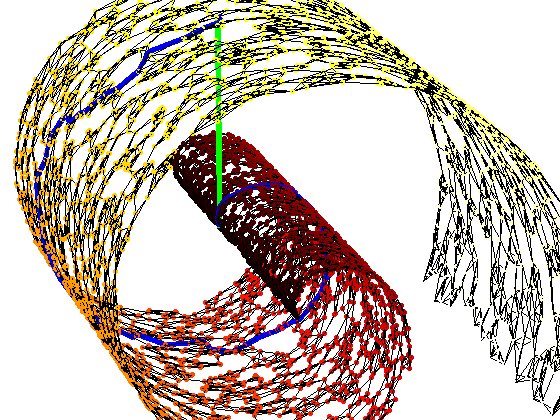
\includegraphics[height=2in]{swiss.png}
\caption{ \small {Data distributed on the "Swiss roll". The geodesic is shown in blue, while the Euclidean distance is shown in green.}}  
\end{figure}
\noindent
An illustration of intrinsic dimension is shown in Figure 1 which depicts an intrinsically two dimensional manifold (known as the Swiss roll) embedded in a three dimensional ambient space.   

\subsection{The Curse of Dimensionality}

	\hspace{5mm} Many practitioners working with high-dimensional data take on a somewhat cavalier approach, hoping to extend common notions in two and three dimensional space to spaces of far higher dimensions. However many so called intuitive notions do not translate to higher dimensions, furthermore some phenomena that are subdued in low dimensional spaces dominate in higher dimensions. Here we summarize some of these phenomena without proof.

The simplest and most famous problem which arises in high dimensional data was coined as the "curse of dimensionality" by Bellman in 1961 \cite{ManLearn}. The curse of dimensionality refers to the simple fact that the number of data points required for an accurate estimate of a probability distribution or manifold structure grows exponentially with the dimension. Therefore as the dimensionality increases, exponentially more points are required to obtain a good estimate of the distribution of the data. This fact underscores the need to incorporate some prior knowledge of the data, which amounts to discovering the constraints that the data is subject to, geometrically this reduces to finding the manifold on which the data lies.  

Another phenomena, which is especially relevant for discrimination in high dimensions is dubbed as the \textit{''concentration phenomenon''} \cite{ManLearn}. It is based on the observation that the mean Euclidean norm of a $D$-dimensional vector grows proportionally to $\sqrt{D}$ however the variance of the Euclidean norm remains roughly constant for a sufficiently large $D$. In other words, as the dimensionality of randomly distributed i.i.d. vectors grows they appear to be all distributed at roughly the same distance from the origin, i.e. on a hypersphere of radius $\mu_{\|y\|}$. This means that using the Euclidean distance between two high dimensional vectors is not an effective discriminative measure.  

Finally, we mention the aspect of low dimensional manifolds embedded in higher dimensional spaces which is potentially the most important in pattern recognition, that is the commonly known notion of geodesic distance. Consider a nonlinear manifold embedded in a higher dimensional space, as is the case illustrated in Figure 1. This is a highly fictitious manifold in the sense that it is not reasonable to expect realistic data to lie on such a smooth manifold, nevertheless we use this example to illustrate an important principle. Suppose that the spatial dimensions represent some features of some objects, for example the three spatial dimensions could represent the length, weight and color of some collection of objects. Suppose further that the yellow points on the outermost side of the manifold denote objects from some category labeled $A$ and the red points denote some other objects from some category $B$. We wish to have some continuous measure of similarity between objects for discrimination purposes. A commonly used measure is the Euclidean distance. In Figure 1 the Euclidean distance between an object in category $A$ and an object in category $B$ is depicted by the straight green line. It is easy to see that this distance is comparable to the distance from the object in category $A$ and other objects in the same category (i.e. other yellow points). This means that the Euclidean distance between points is not a good discriminative measure. On the other hand the geodesic distance between the object in category $A$ and the object in category $B$ is much larger. The geodesic distance is the length of the curve, constrained to lie on the manifold, connecting two points on the manifold. The geodesic is depicted by the blue curve in Figure 1. The figure was generated by constructing a graph in which neighboring points are connected    
by edges, as long as the manifold has relatively low curvature these edges are roughly tangent to the manifold. Geodesic distances can be computed using a standard shortest path algorithm, such as Dijkstra's algorithm. This method of computing geodesic distances is used so called ''Isomap'' nonlinear dimension reduction algorithm \cite{Isomap}.    

\subsection{Dimensionality Reduction} 
The incentive for reducing the dimensionality of data is not only to mitigate the curse of dimensionality but also to obtain a succinct representation of the data based on a smaller set of new variables, sometimes called latent variables. Basically, dimensionality reduction is a mapping from a higher dimensional space, where the data does not "fill" the space, to a lower dimensional space where the data better spans the new lower dimensional space. Such a mapping is, of course, non unique and a mapping which preserves the geometrical or topological structure of the data is preferred. A common criteria for dimension reduction mappings is that distances be preserved. For example, if the Swiss roll in Figure 1 were "unrolled" to a plane by some dimension reduction algorithm then geodesic distances on the original manifold in $\mathbb{R}^3$ would be equivalent to the Euclidean distance computed in $\mathbb{R}^2$. 

\section{Over-complete Bases and Sparse Coding}
Sparse coding seeks to find a representation for some signal (data) $s$ as a linear superposition of a few elements $\phi_i$ from an over-complete basis $\Phi$. In other words $s$ is synthesized as $s = \sum_i \alpha_i \phi_i$, using as few nonzero $\alpha_i$ as possible. If the basis elements are discretized into vectors of finite length, the sparse coding problem can be described using matrix notation. 
\begin{equation}
min \| \alpha \| _0 \mbox{ subject to } \Phi \alpha = s
\end{equation} 
Where $\Phi$ is a "fat" (i.e. there are more columns than rows) matrix which contains the basis elements $\phi_i$ as its columns, and the vector $\alpha$ is a vector of coefficients which we will call the "code" for the signal $s$. If this optimization is carried out only over the coefficients $\alpha$ using a fixed basis this problems is known as the compressive sensing problem \cite{Osher}. The problem is called sparse coding if we allow optimization over the basis $\Phi$ as well as the coefficients. Strictly speaking sparse coding is not a dimension reduction technique because it is a mapping from the original representation of the signal to an even higher dimensional space. However since the coefficients in the new space are constrained to be sparse the signal representation will be some low dimensional hyperplane in the new space. In the terminology of dimension reduction, the latent variables are all $\alpha_i$ such that $\alpha_i \neq 0$ and hence the intrinsic dimension is $P=\| \alpha \|_0$. The sparse coding representation of data is best viewed as a sparse local linear approximation, rather than a global dimension reduction. 

Why $\Phi$ is over-complete? The over-completeness property of $\Phi$ is what allows us to seek sparse solutions. If, for instance, $\Phi$ was an orthogonal basis then we would need every basis element from $\Phi$ to reconstruct $s$ exactly (unless $s$ happened to lie in a subspace of $\Phi$). If $\Phi$ is initially an over-complete random basis then there is a good chance that a few of the random basis elements closely span the data in question. Figure 2 illustrates this situation in two dimensions. The data is distributed on two squares on the line $y=x$, indeed a fair sparse approximation to this data is a single basis element $\phi_i=(1,1)^T$. 
 
\begin{figure}
\centering
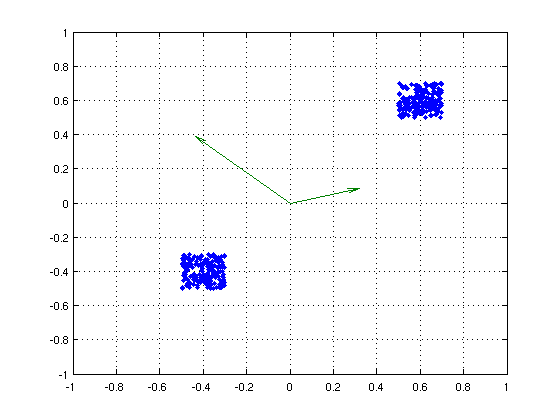
\includegraphics[height=2in]{basis.png}
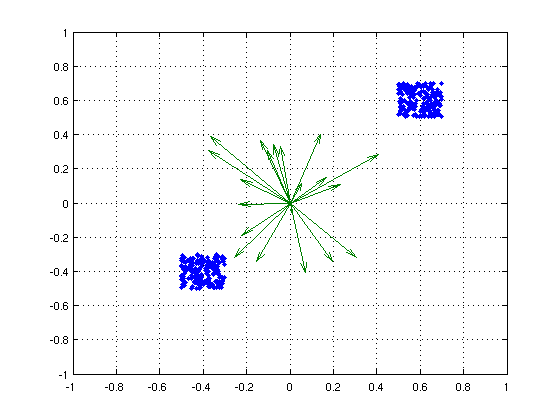
\includegraphics[height=2in]{overcomplete.png}
\caption{ \small {Data is distributed on (very) approximately a one dimensional manifold in two dimensional space. The left figure shows a complete random basis, depicted by the green arrows. The right figure shows an over-complete random basis.}}  
\end{figure}

The optimization in sparse coding is split into two phases. In the first phase an initially random dictionary $\Phi$ is held fixed and a solution to the optimization problem given by Equation 1 is obtained. This is identical to the compressive sensing problem and is called the inference step in sparse coding. In the second phase, the coefficients are held fixed and the dictionary elements are updated. Given Equation 1, it is not clear how to update the basis elements in order to obtain a sparser solution. Furthermore, the $\L^0$ norm implies that the previously defined optimization problem is combinatorial in nature. In the discussion that follows we will reformulate the optimization problem given by Equation 1 to more manageable form and discuss solutions to the sparse coding problem. 
\subsection{The Inference Subproblem} 
The inference step of sparse coding has been an independent and active area of research well before the ideas behind sparse coding were introduced by Olshausen and Field in 1996 \cite{Sparse Coding}. Because the dictionary $\Phi$ is over-complete there are many possible ways to synthesize a given signal $s$ however in the spirit of dimension reduction we seek the sparsest solution. The sparsity criteria acts as a regularizing criteria to the under-determined problem. We will first review some early solutions to this problem, and later introduce the solution based on $\L^1$ regularization which is considered a major breakthrough.

One of the earliest proposed solutions to the inference problem is known as matching pursuit, proposed by Mallat and Zhang in 1993 \cite{25 in BP}. Matching pursuit attempts to synthesize the signal by greedily selecting one element at a time from the basis, which best matches the residual signal at the current iteration. That is, starting from an initial signal approximation $s_0 = 0$ and residual signal $R_0 = s$. At iteration $i$ a single element $\phi_i$ is selected from the basis by computing the maximal inner product $\arg\max_{\phi_i} < R_i, \phi_i>$. The residual is subsequently updated by $R_{i+1} = R_i - \alpha_i \phi_i$ where $\alpha_i = < R_i, \phi_i>$. As noted in \cite{BasisPursuit}, if the dictionary elements are mutually orthogonal, that it is $<\phi_i,\phi_j> = 0$ for $i \neq j$ matching pursuit arrives at the globally optimal solution. Which means that if the $D$-dimensional signal $s$ can be represented by $P<D$ elements from the dictionary $\Phi$ those dictionary elements can be found by matching pursuit. If the dictionary elements are not orthogonal, as is the case for over-complete dictionaries, matching pursuit sometimes fails to yield the sparsest representation. An intuitive example of such a case was presented in \ref{BasisPursuit}, where an over-complete discrete cosine dictionary was used to decompose a signal composed to two sinusoidal signals with closely spaced frequencies. The basis pursuit algorithm choses the first basis element whose frequency is between the two sinusoids. Because of this initial mistake the algorithm is forced to choose basis elements to make "alternating corrections", it misses the twin sine structure of the signal and does not arrive at the optimally sparse representation.

Another approach, proposed by Doubechies \ref{9 in BP} solves the following optimization problem: 
\begin{equation}
min \| \alpha \| _2 \mbox{ subject to } \Phi \alpha = s
\end{equation} 
The $L^0$ norm has been replaced by the $L^2$ norm, which makes the problem much easier not only because the $L^2$ norm is differentiable but because there is a well known closed form solution given by the pseudo-inverse: 

\begin{equation} 
\nonumber 
\alpha = \Phi^T(\Phi \Phi^T)^{-1}s
\end{equation}
Unfortunately there is no reason to expect that solving the problem described by Equation 2 will in any way approximate a solution to Equation 1, and indeed $L^2$ regularization does not lead to sparse solutions but only to solutions whose length (i.e. $\| \alpha \|_2$) is minimized.  

\subsection{$L_1$ Regularization and Basis Pursuit}
A key breakthrough to solving the inference problem came in 1998 when an algorithm called "basis pursuit" was published by Chen, Donoho, and Saunders \cite{BasisPursuit}. The method makes a seemingly trivial change to the matching pursuit problem given by Equation 2. Namely, the $\L^2$ norm is replaced by the $\L^1$ norm yielding the basis pursuit problem: 
\begin{equation}
min \| \alpha \| _1 \mbox{ subject to } \Phi \alpha = s
\end{equation} 
The optimization problem described by Equation 3 can be formulated as a linear program in standard form by introducing the new variables $\alpha^-$ and $\alpha^+$ such that $\alpha = \alpha^+ - \alpha^-$. These new variables can be expressed in terms of the original variables $\alpha$ as $\alpha^+=max(\alpha,0)$ and $\alpha^-=max(-\alpha,0)$. The equivalent linear program can now be written as: 
\begin{equation} 
\nonumber
min \begin{pmatrix}1,1 \end{pmatrix} \begin{pmatrix} \alpha^+ \\ \alpha^- \end{pmatrix} \mbox{ subject to } \begin{pmatrix} \Phi, -\Phi \end{pmatrix} \begin{pmatrix} \alpha^+ \\ \alpha^- \end{pmatrix} = s
\end{equation}  
The above linear program can be solved using well known algorithms such as simplex or interior-point methods \cite{Nocedal and Wright}. Moreover, the authors of \cite{BasisPursuit} noticed that the $L^1$ criteria lead to sparse solutions, the rigorous proof of exactly why this happens was not obtained until 2006 by 
the combined efforts of Donoho, Candes, Romberg and Tao \cite{Compressive Sensing}. The complete proof is beyond the scope of this work, however we appeal to the solution of Exercise 2.3 \cite{David Eigen} for an intuitive glance at why this happens. In Exercise 2.3 we were asked to determine the solution to the following optimization problem: 
\begin{equation} 
min~ e^T x \mbox{ subject to } a^Tx \geq \beta \mbox{ and } x \geq 0 
\end{equation}
Where $a \in \mathbb{R}^n$, $\beta$ is a positive scalar, and $e$ is an $n$-vector of ones. Note that $x$ plays the role of $\alpha$ in the previously defined notation. If the inequality constraint is transformed to an equality constraint, this problem becomes a special case of the basis pursuit problem described by Equation 3 in the first orthant, with only one constraint. The vertices of the feasible region are given by $x_i = \frac{\beta}{a_i} e_i$ where $a_i$ is the $i^{th}$ component of $a$ and $e_i$ is the $i^{th}$ coordinate axis, for each $a_i >0$. For those $a_i \leq 0$ there is either no intersection with the coordinate axis or the intersection occurs in the infeasible region. The value of the objective $e^Tx_i$ at the vertices is 
\begin{equation} 
\nonumber 
e^T x_i = e^T \left( \frac{\beta}{a_i} e_i \right) = \frac{\beta}{a_i}
\end{equation} 
Clearly the objective is minimized when $a_i$ is largest. Let $k = argmax_i~a_i$, i.e. $k$ denotes the set of indexes with the largest positive $a$ component, and let $a^* = max~a_i$. Then any point point in the affine subspace spanned by the $k$ vertices yields the same value for the objective function, and the solution is: 
\begin{equation} 
\nonumber
x^* = \sum_k \frac{\beta}{a^*} s_k e_k, ~~~ \sum_k s_k =1, ~~~ s_k \geq 0
\end{equation}    
A consideration of the dimensionality of $x^*$ reveals the significance of this result. If $argmax_i~a_i$ is unique then the set $k$ includes only one index and thus the solution is sparse. In what case will $argmax_i~a_i$ be unique? Compressive sampling and the initialization in sparse coding achieve this by selecting the basis vectors, which act as the constraints, at random.

Due to the potential presence of noise in the signal $s$ we may not want to solve the basis pursuit problem directly. Assuming that the signal does indeed contain random additive noise, as is common to almost all physically acquired data, and if the noise component is independently distributed, it will span the full dimensionality. No dimension reduction would be possible if we require that the signal as well as the noise be reconstructed exactly. Assuming that the noise amplitude is relatively small as compared to the signal amplitude, i.e. $s = s^* + \nu$, where $s^*$ is the true signal and $\nu$ is some additive noise term, we assume that $\|\nu\|_2 << \|s^*\|_2$. With this assumption we can assert that $\|s-s^*\|_2 << \|s-\nu\|_2$, which means that $s^*$ is a much better estimate for $s$ than $\nu$ in the $L^2$ sense. To avoid enforcing the requirement of reconstructing the noise term, the hard constraints of the original problem are relaxed and used as a regularizing term in the following modified problem:   \\
\begin{equation}
\min_{\alpha} \frac{1}{2} \|s - \Phi \alpha \|_2 ^2 + \lambda \| \alpha \|_1
\end{equation} 
Where the parameter $\lambda$ controls the relative importance between the reconstruction and sparsity term. The above problem is called "basis pursuit de-noising" (BPDN) in \cite{BasisPursuit}, however this formulation was actually proposed two-years prior to basis pursuit in \cite{Lasso} and \cite{Sparse Coding}. An early solution to the BPDN problem was by gradient descent, also proposed in \cite{Sparse Coding}. However more sophisticated algorithms were developed in recent years such as the "iterative shrinkage and thresholding" (ISTA) and FISTA (Fast ISTA) algorithms \cite{ISTA}, \cite{FISTA}. According to \cite{Osher}, the basic idea behind ISTA can be intuited by considering the one dimensional problem: 
\begin{eqnarray}
\nonumber
\min_x~ E(x)  =  \frac{1}{2}(x - f)^2 + \lambda|x| \\
\nonumber 
\nabla E(x) = 0 \mbox{ leads to }\\
\nonumber 
(x-f) + \lambda sgn(x) = 0
\end{eqnarray}
Since $E(x)$ is convex, a unique solution can be obtained by solving the above equation. For the case when $x>0$ the equation above implies that $x = f - \lambda > 0$, and when $x<0$ the solution is $x=f+\lambda<0$. This leads to the introduction of the so called shrinkage function $x = shrink(f,\lambda)$.  
\begin{figure}[ht]
\centering
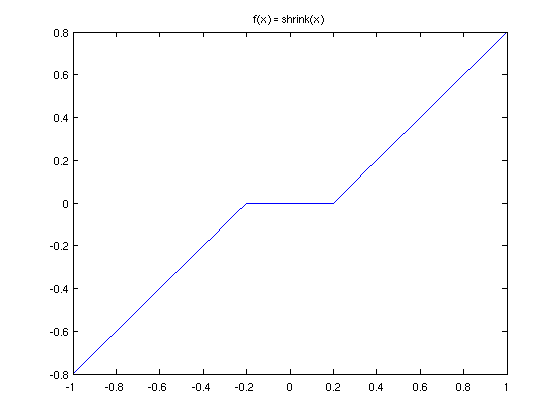
\includegraphics[height=2in]{shrink.png} 
\end{figure}\\
When the independent variable $x$ is multidimensional as in the case of $\alpha$, since the $\| \alpha \|_1$ term is separable, the shrinkage solution can be applied component-wise to $\alpha$. This approach, known as ISTA, is a coordinate descent type algorithm. It was shown in \cite{FISTA} that the shrinkage update can be applied to all the components of $\alpha$ at the same time, and this approach is known as FISTA. In the work that follows we will use the FISTA solution for $\alpha$ given by the update: 
\begin{equation}
\alpha_{k+1} = shrink(\alpha_k - \eta_1 \nabla_{\alpha_k}E) 
\end{equation}   
Where $E(\alpha,\Phi) = \frac{1}{2} \|s - \Phi \alpha \|_2 ^2$, and  $\eta_1$ is the step size of the update. 

\subsection{Optimization of the Basis}
The second phase of optimization in sparse coding is the basis update. Given that the set of optimal coefficients $\alpha^*$ have been found using Equation 6, the basis is updated by solving: 
\begin{equation}
\min_{\Phi} \frac{1}{2} \|s - \Phi \alpha^* \|_2 ^2 
\end{equation} 
This is for a single fixed input vector $s$, however normally a dataset is composed of many signals which constitute the manifold. Thus we seek find that best basis that sparsely reconstruct all of these signals. One way to describe this objective is by the average squared reconstruction error criteria: 
\begin{equation}
\min_{\Phi} \frac{1}{N}\sum_{i = 1} ^N \frac{1}{2} \|s_i - \Phi \alpha_i^* \|_2 ^2 
\end{equation}
Although we wish to minimize the reconstruction error over all signals, the gradient of Equation 8 is computed with respect to only one signal at a time and the basis elements are updated accordingly. This approach is called "stochastic gradient descent" \cite{Yann} and is heavily used in machine learning. The stochastic gradient update has many advantageous properties, especially if the dataset contains redundant samples. Using the stochastic gradient the basis update is: 
\begin{equation}
\Phi_{k+1} = \Phi_k - \eta_2 (s_i - \Phi_k \alpha_i^*)\alpha_i^{*T}
\end{equation} 
Because the shrink function is applied to the $\alpha$ coefficients prior to the basis update, many of the less important basis elements for reconstruction will not be updated. In this sense, sparse coding finds a basis which is resilient to sparsification. 
\newpage
\section{Results and Discussion} 
Sparse coding was first applied to natural imagery (images of foliage were used) in order to find a basis which best sparsely represents natural images. The basis which is obtained by sparse coding is remarkably similar to the receptive fields of simple cells in the mammalian cortex \cite{Sparse Coding}, which in turn are very similar to the Gabor wavelet basis. In this subsection the results from these experiments are presented and some applications are discussed. The sparse coding basis for image patches extracted from natural images is obtained by following the optimization procedure outlined in this paper. The dimensions of each patch is 16 by 16 pixels. The patches are reshaped into columns and used as the signal variables $s_i$. The basis is composed of 400 initially random, 16 by 16 basis elements, which are also reshaped and comprise the columns of $\Phi$. Not that there are 400 basis elements in a 256 dimensional space thus the basis is over-complete.   

\begin{figure}[ht]
\centering
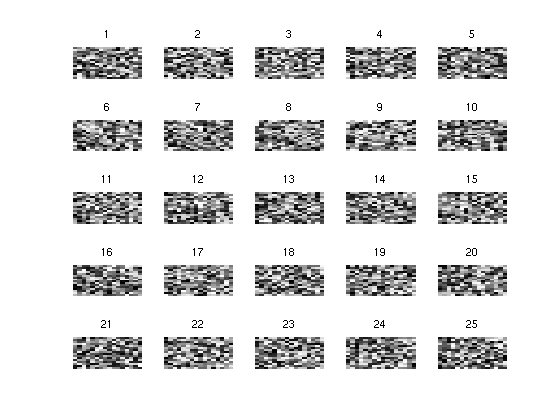
\includegraphics[height=2in]{random.png}  
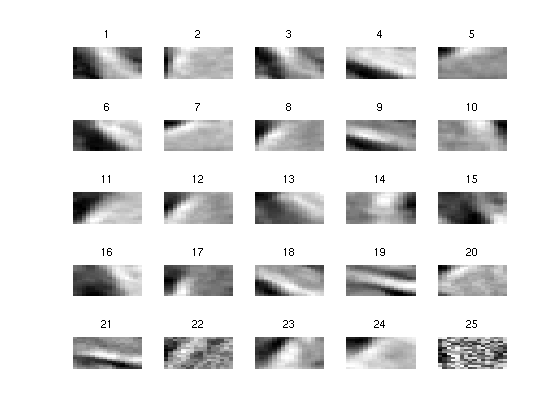
\includegraphics[height=2in]{iter1.png} 
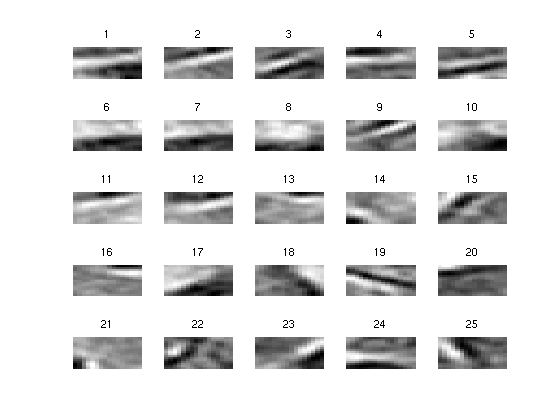
\includegraphics[height=2in]{iter6.png}
\caption{ \small{Top Left: Initialized random basis, Top Right: Top 25 basis vectors after 19200 image patch presentations, Bottom: Top 25 basis vectors after 115200 image patch presentations}} 
\end{figure}
\newpage
\noindent
The results of sparse coding on natural image patches are shown in Figure 3. Of the 400 basis elements, 25 with the largest inner product with the image patches are displayed. The initially random basis elements are shown at the top left. After 19200 patch presentations most basis elements resemble broad edge detectors. After 115200 presentations the basis elements become more specialized and Gabor wavelet-like structure emerges.

Aside from a mathematical model for the low-level mammalian visual processing system, sparse coding has found applications in machine learning in recent years. The basis produced by sparse coding is used to initialize deep learning machines, such as neural networks with multiple layers \cite{DeepLearning}. Due to the huge parameter space of these models the learning process converges very slowly, or does not converge to anything sensible at all without this initialization.

  \begin{thebibliography}{1}

  \bibitem{EncyclopediaBritannica} Encyclopedia Britannica Online, Search Query: Computer Vision

  \bibitem{ManLearn} John A. Lee and Michel Verleysen {\em Nonlinear Dimensionality Reduction}, Springer 2007 

  \bibitem{Isomap} J. B. Tenenbaum, V. de Silva and J. C. Langford {\em A Global Geometric Framework for Nonlinear
Dimensionality Reduction} Science 290 (5500): 2319-2323, 22 December 2000 

  \bibitem{Osher} Yingying Lee and Stanley Osher {\em Coordinate Descent Optimization for $\l^1$ Minimization with Applications to Compressed Sensing; a Greedy Algorithm} UCLA CAM Report
  
  \bibitem{Sparse Coding} Bruno A. Olshausen and David J. Field{\em Emergence of simple-cell receptive field properties by learning a sparse code for natural images} Nature 381, 607 - 609 (13 June 1996)
  
  \bibitem{25inBP} S. Mallat and Z. Zhang {\em Matching Pursuit in a time-frequency dictionary} IEEE Transactions on Signal Processing, Issue 41 (1993)
  
  \bibitem{BasisPursuit} S. S. Chen, D. L. Donoho, and M. A. Saunders {\em Atomic Decomposition by Basis Pursuit}  
  
  \bibitem{9 in BP} I. Daubechies, {\em Time-frequency localization operators: a geometric phase-space approach}, IEEE Transactions on Information Theory, Issue 34 (1988)  
  
  \bibitem{Nocedal and Wright} Jorge Nocedal and Stephen J. Wright {\em Numerical Optimization}, Springer 2006  
  
  \bibitem{CompressiveSensing} E. J. Candes, J. Romberg and T. Tao. {\em Stable signal recovery from incomplete and inaccurate measurements} Comm. Pure Appl. Math., 59 1207-1223
  
  \bibitem{David Eigen} David Eigen {\em Numerical Optimization Homework 2,} 2011  
  
  \bibitem{Lasso} Tibshirani, R. (1996). {\em Regression shrinkage and selection via the lasso.} J. Royal. Statist. Soc B., Vol. 58, No. 1, pages 267-288).

  \bibitem{FISTA} Amir Beck and Marc Teboulle {\em A Fast Iterative- Thresholding Algorithm for Linear Inverse Problems} SIAM J. Imaging Science Vol.2 No.1
  
  \bibitem{Yann} Yann LeCun, Leon Bottou, Genevieve B. Orr, and Klauss-Robert Muller {\em Efficient BackProp} AT\&T Labs Technical Report
  
  \bibitem{Vision} Richard Szeliski {\em Computer Vision}, Springer 2011
  
  \bibitem{DeepLearning} Itamar Arel, Derek C. Rose, and Thomas P. Karnowski {\em Deep Machine Learning: A New Frontier in Artificial Intelligence} 

  \end{thebibliography}

  
  
  
  

\end{document}












